\documentclass[simplex.tex]{subfiles}
% DO NOT INCLUDE PREAMBLES/PACKAGES HERE!!
% packages are inherited from preamble.tex; you can compile this on its own
\begin{document}
\subsection[ndviz]{ndviz}

The vast majority of current high resolution imaging techniques in neuroscience are either 3-dimensional or contain a 3-dimensional component (e.g. 3-d data over time). Visualization of data produced by said techniques has traditionally been confined to the three canonical planes; $xy$, $yz$, and $xz$. However, advancements in Web graphics rendering have made dynamic, 3-dimensional visualization possible in modern Web browsers. Using WebGL, code running in a users Web browser can access the end users Graphics Processing Unit (GPU), taking advantage of specialized graphics hardware present in most modern desktops, laptops, and even smart phones. 

Using WebGL for dynamic rendering improves both the performance and capability of a graphical Web application. To that end, we have integrated \href{https://github.com/google/neuroglancer}{Neuroglancer}, a Web visualization tool built for 3-dimensional data, into NeuroDataViz. Neuroglancer has provided us with a baseline 3-dimensional rendering tool, which we can use for specialized features (e.g. dynamic false coloring). By building on a common framework, we can contribute features back to the neuroscience community as well as take advantage of new features developed by our collaborators (or even other neuroscience users). 

With this new version of NeuroDataViz, we can visualize all of our existing data in the three canonical planes mode. We are now working to build 3-dimensional meshes, both for annotated Electron Microscopy data and for thresholded Light Microscopy data. A sample of EM meshes is available in the figure below. We are now developing tools for automatically generating 3-d meshes (shapes) for both datatypes on-demand as the user makes a selection in the 3-d view.  


%%%   EXAMPLE FIGURE BLOCK
\begin{figure}[!h]
\begin{cframed}
\centering
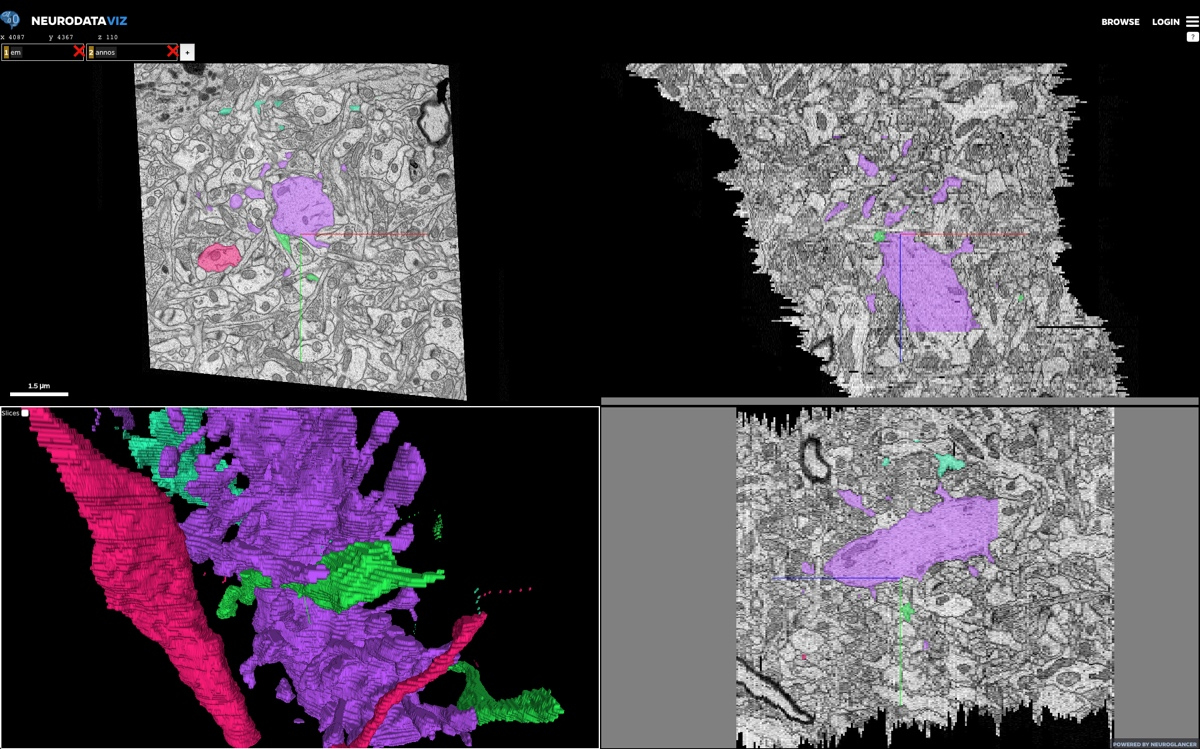
\includegraphics[width=0.95\textwidth, height = 3in]{../../figs/ndviz3d_fig.jpg}
\caption{NeuroDataViz, powered by Neuroglancer with pre-computed meshes
  displayed in 3-d. Data from Harris et al. ``A resource from 3D
  electron microscopy of hippocampal neuropil for user training and tool
  development,'' Nature Scientific Data 2015.}
\label{fig:name}
\end{cframed}
\end{figure}

\clearpage
\end{document}
